\section{Methodology and Implementation}
% What were the methods used?
% How was the problem designed?
% Driving concepts
% Equations
% Figures

A modular, agent-based is an ideal approach for solving complicated
physics-dependent supply chain problems involving material routing, facility
deployment, regional and institutional hierarchies.

\subsection{Framework Structure}
% (OO, cpp, xml, backends, inheritances, mixins, generic apis, etc.)

Agent-based modeling is inherently object oriented. 

The core of the simulator creates a set of key classes on which agent plugins 
are based. In addtion, a set of key tools are also provided, to enrich the API 
and provide a robust suite of behaviors for the developer.

<diagram of core, modules, toolkit, etc>

Agent plugins utilize the generic core API to interact with one another. 
Mainly they do this by trading resources. 

<diagram of black box facilities>

\subsection{Cluster-Ready Software}

\Cyclus is primarily written in \texttt{C++}, and support is currently provided
for Linux-based (including Ubuntu and OSX) platforms. Furthermore, the core
infrastructure and related archetypes are free and open-source, BSD-3-clause
licsened. No part of \Cyclus is proprietary or based on commercial, off the
shelf (COTS) software. Accordingly, it can be easily deployed on large compute
systems, such as high-throughput computing (HTC) systems.

Cyclopts (\TODO{cite}), a proof of principle design and implementation of such a
system, uses UW-Madison's HTCondor HTC infrastructure to perform sensitivity
studies on \Cyclus' resource exchange optimization solvers. To date, it has been
used run over $10^4$ jobs, or (\TODO{compute time}) total compute hours, using
the \Cyclus library via its resource exchange API.

\subsection{Dynamically Loadable Libraries}
% (diagram)

A key innovation that has previously not been implemented in nuclear fuel cycle 
simulators in the literature is implementing this generic API and modular 
architecture into a suite of dynamically loadable ``plugin'' libraries.
This is implemented largely through a clean API and a modern build system.

Dynamically-loadable libraries are the primary mechanism for extending \Cyclus' capability. 
This approach provides encapsulation: the core of the code operates
completely independently from the individual plugin libraries. Thus, any
customization or extension is implemented only in the loadable
library. 

This approach allows efficient, targeted contribution to the ecosystem of libraries.  The 
scientist-developer can focus on generating a model within their
sphere of expertise, while relying on the model contributions of others to fill 
in the other technologies.  This strategy also allows individual developers to
explore different levels of complexity within their archetypes, including
wrapping other simulation tools as loadable libraries within the \Cyclus
framework.

A secondary benefit is the ability for
contributors to choose different distribution and licensing strategies
for their contributions. By allowing models to have varied
availability, the security concerns of developers can be
assuaged (See Figure \ref{fig:modifiedopen}).

\begin{figure}[htbp!]
\begin{center}
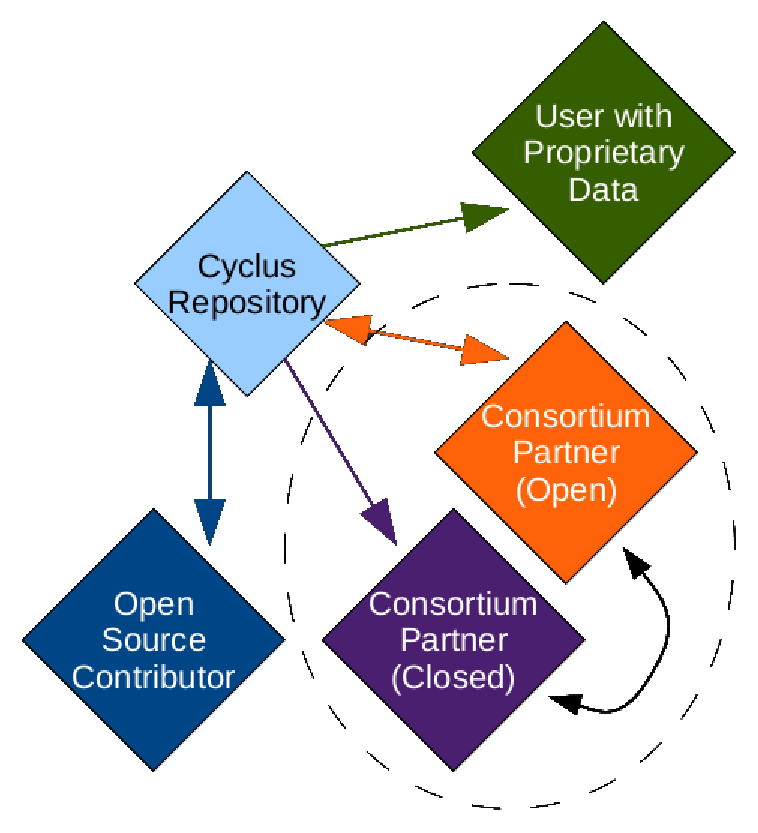
\includegraphics{./images/modifiedopen.eps}
\end{center}
\caption{The \Cyclus framework enables fully open, partially open, and fully
closed collaborations\cite{wilson_cyclus:_2012}.}
\label{fig:modifiedopen}
\end{figure}

In particular, since the clean plugin architecture loads libraries without any
modifications to the \Cyclus kernel, closed-source archetypes can be used with
the simulator alongside open-source archetypes. This architecture
allows closed-source libraries (e.g., those representing sensitive nuclear
processes and subject to export control) to be developed and licensed privately.

This last benefit of dynamically-loadable libraries addresses
another goal of \Cyclus: ubiquity amongst its potential user base. By
engineering \Cyclus to easily handle varying levels of complexity, a single
simulation engine can be used by both users interested in big-picture policy
questions as well as users focused on more detailed, technical
analyses.

\subsection{Agent Interchangability}\label{sec:interchangeability}

A key compontent of the \Cyclus kernel architecture is the ability for
implementations of actors in a given simulation to be easily
interchanged. Critically, this novel functionality enables the comparison
between agent implementations. For example, a low-physics-fidelity
implementation of a reactor can be compared to an implementation with higher
physics fidelity, allowing an analyst to discern the effect of reactor physical
fidelity on a given fuel cycle. 

Interchangability is accomplished by providing APIs that define agent-to-agent
interaction and agent-to-environment interaction, primarily through the
\Class{Agent} and \Class{Trader} interfaces. The \Class{Agent} interface
provides a notion of parent-child hierarchichal relationship, where parents can
choose to \textit{build} child agents and \textit{decommission} child
agents. The \Class{Trader} interface allows agent-agent interaction through the
trading of \Class{Resource}s. Usabe archetypes in a \Cyclus simulation must
implement the \Class{Agent} interface and may optionally implement the
\Class{Trader} interface. For example, a \Class{Region} implements only the
\Class{Agent} interface, whereas a \Class{Facility} implements both the
\Class{Agent} and \Class{Trader} interface, allowing any \Class{Facility} to
trade with another \Class{Facility}.

\subsection{Regions, Institutions, and Facilities}

\Cyclus provides a novel representation of entities in the nuclear fuel cycle,
including facilities, institutions managing those facilities, and regions. While
some simulators (\TODO{cite DESAE}) have provided a notion of static regional
effects, \Cyclus allows for both regions and institutions to be first-class
actors in simulated fuel cycles.

The basic interaction models for each entity is implemented by a corresponding
archetype class in \Cyclus, i.e., the \Class{Region} class, \Class{Institution}
class, and \Class{Facility} class. Archetype developers can then build on the
provided functionality by subclassing the appropriate class.

\Cyclus implements a Region-Institution-Facility (RIF) relationship through the
parent-child hierarchy described in \S \ref{sec:interchangeability}, where
regions are the parents of institutions which are, in turn, the parents of
facilities. In other words, RIF hierarchies form a directed acyclic graph (DAG),
with regions as root nodes and facilities as leaf nodes.

Two primary consequences arise from this structure. First, institutions are
responsible for building and decommissioning facilities. Accordingly, advanced
logic regarding building and decommissioning can be obtained by subclassing the
\Class{Institution} interface. Second, the \Class{Facility} class implmenets the
\Class{Trader} interface, and thus institutions and regions, respectively, can
adjust the resource flow preferences of their managed facilities. Importantly,
this novel capability allows for the modeling of preferential regional trading
of resources (e.g., tariffs) as well as preferential institutional trading
(e.g., long-term contracts).

Although concept of the RIF hierarchy is provided, the \Cyclus kernel is
really designed to handle hierarchies of arbitrary depth.  It is just as easy
to run a simulation without regions and institutions (i.e.  only facilities)
or a simulation having archetypes that are the parents' of regions.  By
convention, institutions are mainly responsible for facility deployment, but
any archetype can have access to \Cyclus' agent deployment mechanism.  It easy
to implement agents that deploy copies of themselves, or that schedule their
own decommissioning.  Because regions, institutions, and facilities are all
just agents, they can all be implemented to exercise the full set of features
offered by the \Cyclus kernel.

\subsection{Resources and Materials}
% Resources, Materials (note isotope tracking, decay behavior)

TODO: add blurb about discrete agent/facility tracking.

In Cyclus, agents can transfer discrete resource objects between each other.
Cyclus supports two types of resources:

\begin{itemize}

  \item Materials: These represent typical nuclear materials with
      nuclide-based compositions.

  \item Products: These can represent any user-defined thing - e.g. carbon
      credits, build permits, employees, etc.

\end{itemize}

All operations performed on every resource object (splitting, combining,
decay, etc.) are tracked in detail.  This information includes the creating
agent for when resources are newly created and introduced into the simulation.
The parentage of each resource is also tracked. This makes it possible to
follow the travel history of discrete resource objects as they are transferred
between agents.

The \Cyclus kernel has built-in experimental support for decay calculations.
Materials "remember" the time since their last decay and agents are free to
invoke the decay function on them as desired to decay them to the current
simulation time.  Cyclus can currently operate in 2 decay modes with 2 other
modes likely to be added in future releases:

\begin{itemize}

    \item "manual" (currently implemented) is the default mode just described
        where agents decay materials as needed.

    \item "never" (currently implemented) globally turns off all decay.
        Materials' decay function does nothing.

    \item "periodic" (future) automatically decays all materials in a
        simulation with some fixed frequency.

    \item "lazy" (future) decays any material whenever its composition is
        viewed (e.g. when an agent queries information about a material's
        $^{239}$Pu content).

\end{itemize}

In order to avoid excess decay calculations, when a material's decay function
is invoked, the material checks to see if it contains any nuclides with decay
constants that are significant with respect to the time delta for the current
decay operation.  If all the decay constants are not significant, no decay
calculation is performed and the material remains unchanged.  This error does
not accumulate because the next time the material's decay function is invoked,
the time delta will be larger. \TODO{want more detail on this decay shortcut?}
\TODO{describe decay algorithm and how it might be improved}.

\Cyclus has no notion of "tracked" nuclides.  In cyclus, a  material's
composition represents an arbitrarily large list (potentially thousands) of
nuclides.  Agents are free to treat nuclides present in materials any way they
please - including ignoring them.  It is the responsibility of archetype
developers to choose how to handle potentially full-fidelity compositions.

In large simulations there may be many material objects changing frequently.
Material decay can also contribute significantly to such changes.  In order to
help avoid unnecessary runtime performance and database space impacts,
compositions in Cyclus have some special features.  Compositions in Cyclus are
immutable.  This immutability allows multiple material objects to all hold
references to the same composition object safely.  When operations are
performed on a material that don't change the composition, any new resulting
materials hold a reference to the same, originating composition object.
Although the decay operation generates a new, separate composition (preserving
immutability), a reference to the new composition is placed in a cache shared
by the new an originating compositions. The next time the originating
composition is decayed, this cache will be checked for a prior calculation
with the same cumulative decay time.  If one exists, the cached composition is
used.  This cache is shared by all compositions that transitively come from
the same origin.  Composition immutability in concert with decay history
caching help eliminate many redundant decay calculations in addition to
reducing the total number of composition objects.  Since each composition
object is only recorded in the database once, significant space savings also
occurs. \TODO{do we want a diagram helping show this composition caching?}

\subsection{Toolkit}

In addition to the core functionality of the \Cyclus kernel, which is focused on
the minimal set of capabilities needed to implement an agent-based simulation
with dynamic resource exchange, a toolkit is provided that assists developers
and users with related simulation and nuclear engineering tasks. The toolkit is
an activly developed module module of \Cyclus, with a primary forward-looking
focus on supporting interesting \textit{in situ} (i.e., in simulation) and
\textit{ex situ} (i.e., post-processing) metric analysis tools. 

\subsubsection{Simulation Tools}

A series of utility classes are provided to support demand-constrained agent
(e.g. facility) deployment. Symbolic function representations of linear,
expontential, and piecewise functions are supported via the
\Class{SymbFunctionFactory} class. Such functions are used with other toolkit
classes to determine commodity demand (e.g., power demand) from user input. Four
mixin classes provide the basis for in-simulation deployment determination:
\Class{CommodityProducer}, \Class{CommodityProducerManager}, \Class{Builder},
\Class{BuildingManager}. The \Class{CommodityProducer} class provides an
interface for querying the \textit{prototypes} which have some nameplate
capacity to produce a given commdity, and the \Class{CommodityProducerManager}
provides an interface for registering \Class{CommodityProducer}s and querying
the current capacity (supply) of a commodity. The \Class{Builder} class provides
an interface for querying which prototypes can be built and interacts with the
\Class{BuildingManager}, which orders prototypes to be built. The
\Class{BuildingManager} uses a simple minimum cost algorithm to determine how
many of each prototype, $y_i$, to build given a demand, $\Phi$, capacities,
$\phi_i$, and costs $c_i$.

\begin{equation}
\begin{aligned}
 \min & \sum_{i=1}^{N}c_i y_i \\
 s.t. & \sum_{i=1}^{N}\phi_i y_i \ge \Phi \\
      & n_i \in [0,\infty) \:\: \forall i \in I, \:\: y_i \:\: \text{integer} 
\end{aligned}
\end{equation}

\subsubsection{Nuclear Engineering Tools}

The \Cyclus toolkit provides two useful modules for querying \Class{Material}
objects regarding physical parameters. First the \Class{MatQuery} module
provides a basic querying API, including the atom and mass fractions of
nuclides, the number of moles of a nuclide in a material, and also the amount of
aggregate nuclides, i.e., a \Class{Composition}, in a material. The
\Class{enrichment} module provides an API for determining enrichment-related
parameters of a material, including the separative work units (SWU) and natural
uranium required to enrich a material given provided feed, product, and tails
assays.

\subsection{Cycamore}
% base modules

Cycamore contains a number of useful facility models that are a mere base-set.
Additional modules are needed for interesting fuel cycle simulation. However,
simple, once-through fuel cycles can be generated with Cycamore and Cyclus alone.

<diagram of a possible Cycamore-only simulation>
